\documentclass{article}
\usepackage[top=2.54cm, left = 2.54cm, right=2.54cm, bottom=2.54cm]{geometry}

\usepackage{amssymb}
\usepackage{multicol}
\usepackage{amsmath}
\usepackage{graphicx}
\usepackage{booktabs}
\usepackage{verbatim}

\begin{document}

\begin{center}
\textit{\Large{Classical Hydrostatic Equilibrium Equation Derivation}}\\[0.25cm]
\large{Dr. Omair Zubairi}\\
\end{center}

\vspace{0.5cm}
\noindent Hydrostatic equilibrium in stars deals with a balance of the inward force of gravity with the outward push of pressure. Hydrostatic equilibrium is the reason stars do not implode or explode at random. Classically hydrostatic equilibrium is described as

\begin{equation}
 \label{eq:dpdr1}
\dfrac{dP}{dr}=-\dfrac{\epsilon(r)M(r)}{r^{2}}~,
\end{equation}
where $P$ is the pressure, $\epsilon$ is the energy-density, $M$ is the mass, and $r$ is the radius and where the natural mathematical units of $G=c=1$. The derivation of Eq.~\eqref{eq:dpdr1} is a great way to understand some of the basic fundamentals of stellar structure.\\

\noindent Lets begin by considering a volume element with area $dA$, length $dr$, a distance $r$ fromthe center of a start shown in the figure below.

\begin{figure}[ht]
\begin{center}
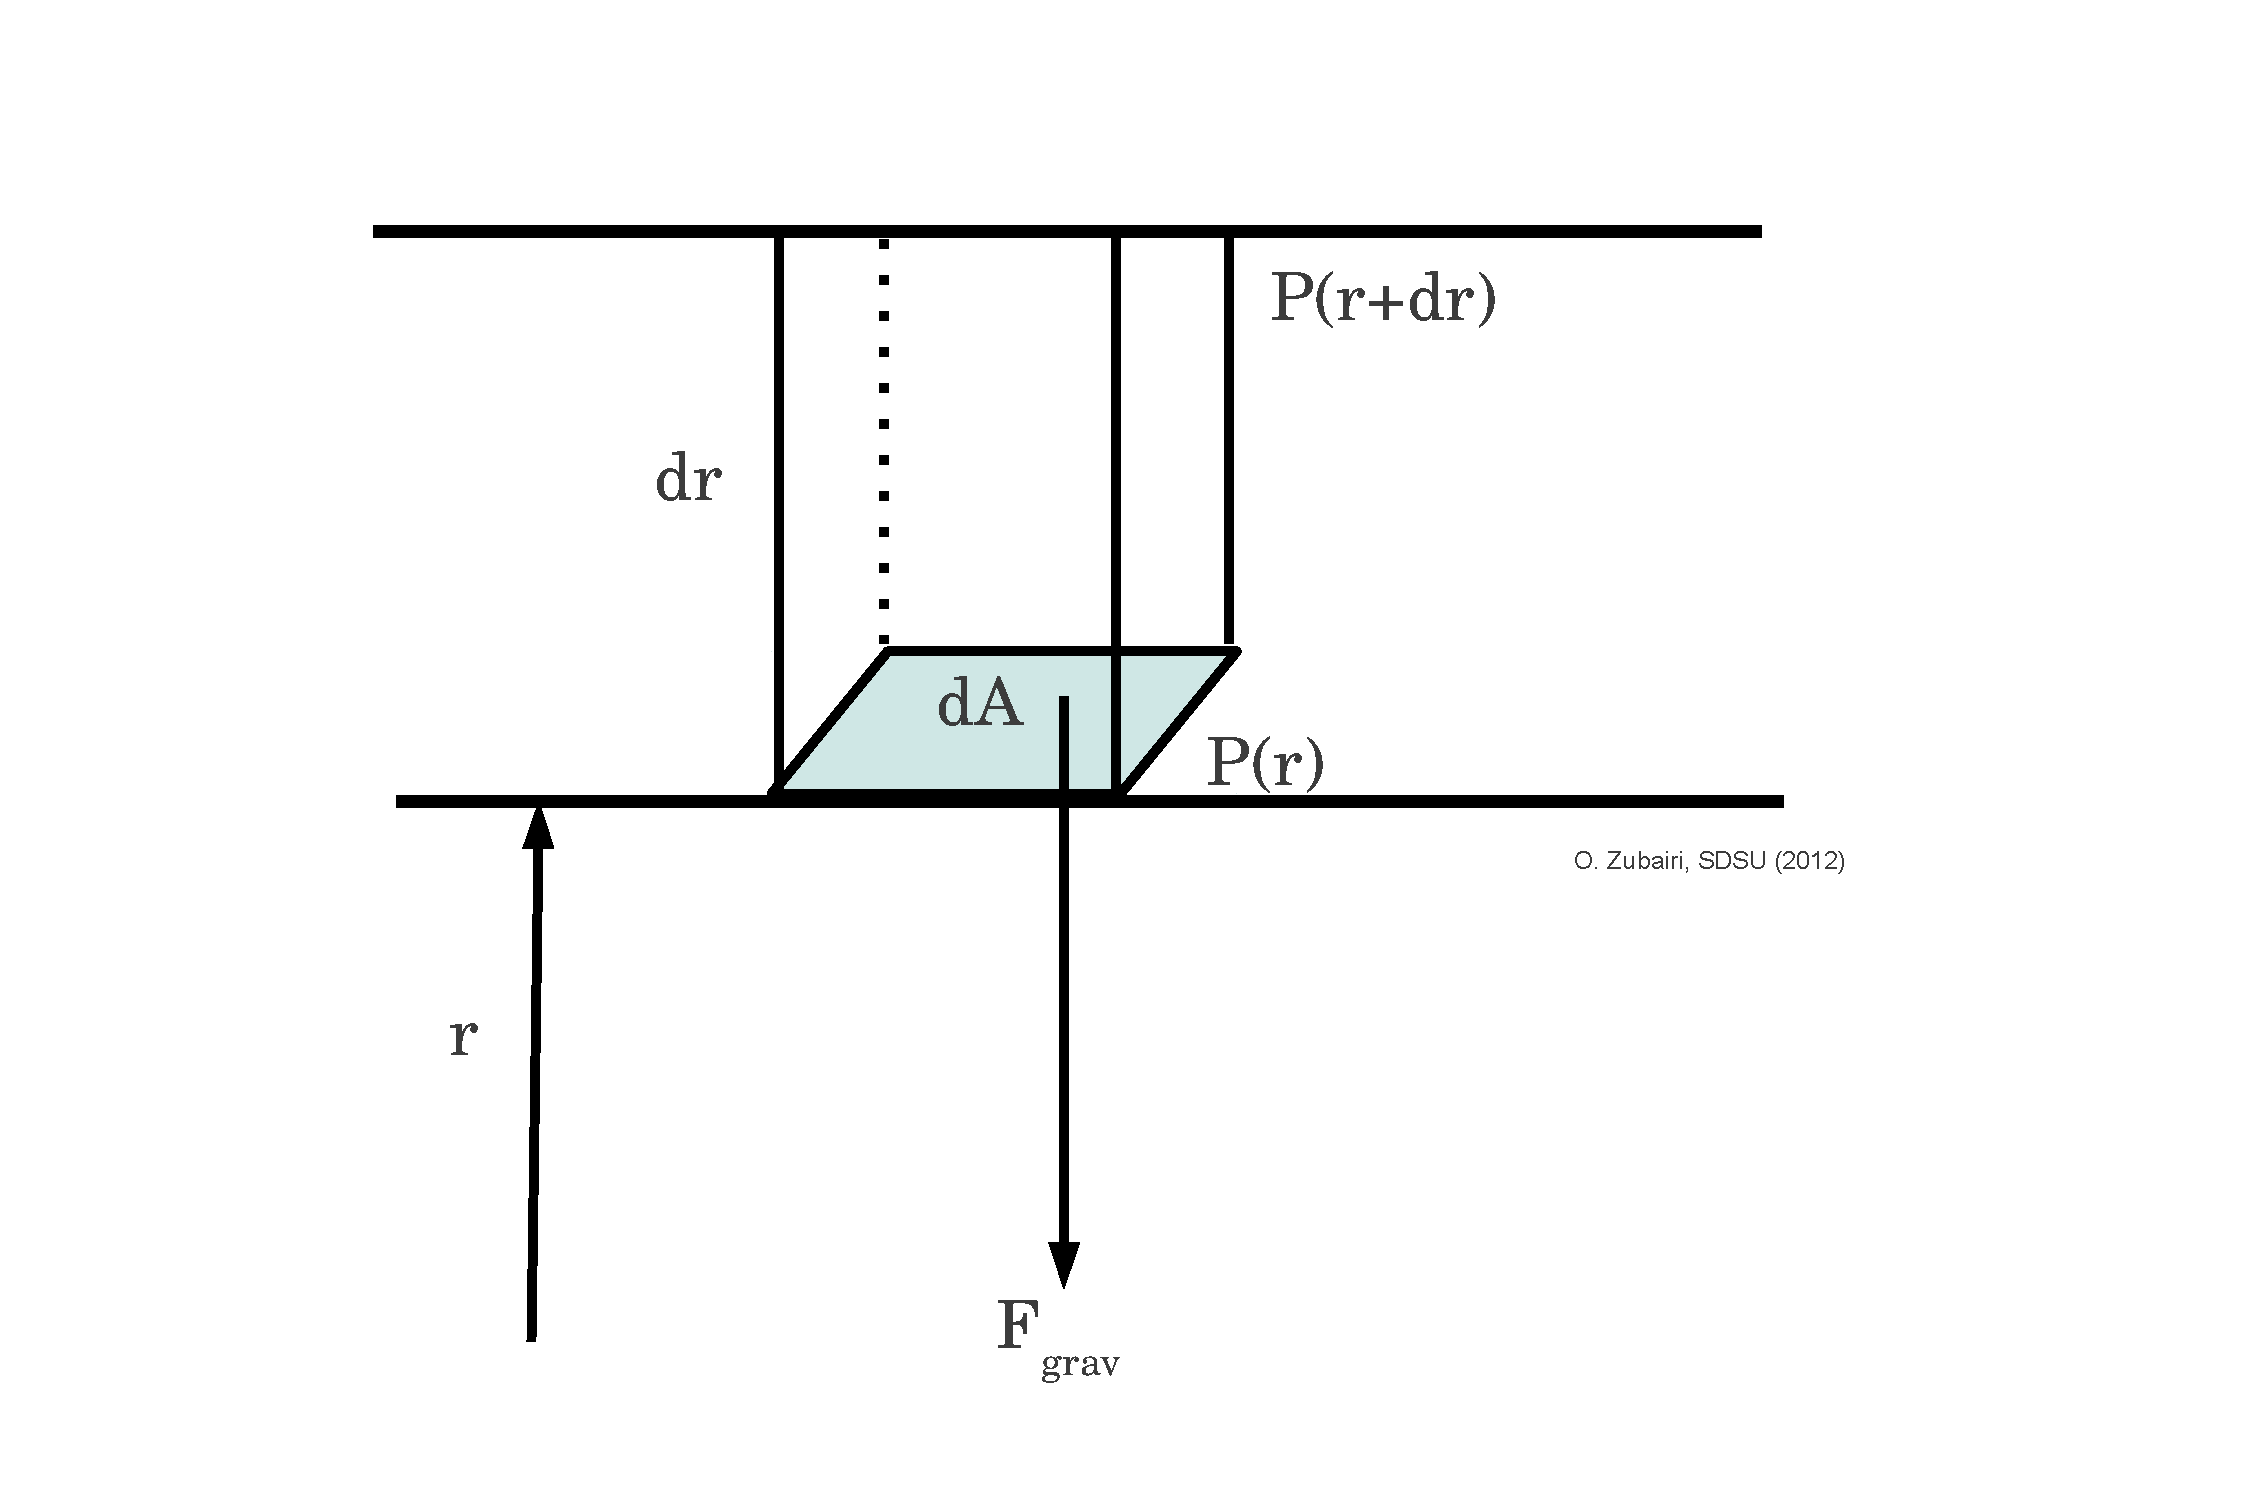
\includegraphics[scale=0.5]{equil.ps}
\caption{\label{fig:dpdr} Volume Element}
\end{center}
\end{figure}
The properties (i.e. Density, Volume, and Mass) of this volume element are as follows:

\begin{itemize}
\item Density: $\rho(r)$
\item Volume: $dAdr$
\item Mass: $dm=\rho(r)dAdr$ (remember that $\rho = \frac{m}{V}$)
\end{itemize}
Next, we need to consider what is $\vec{F}_{grav}$ (force of gravity) acting on the volume element... Its is simply

\begin{equation}
 \label{eq:force1}
F_{grav}=-\dfrac{GM(r)dm}{r^{2}}~.
\end{equation}
Substitute $dm$ into Eq.~\eqref{eq:force1} to obtain 

\begin{equation}
 \label{eq:force3}
F_{grav}=-\dfrac{GM(r)\rho(r)dAdr}{r^{2}}~.
\end{equation}
Define the quantity

\begin{equation}
\label{eq:alpha}
\alpha(r)=\dfrac{GM(r)}{r^{2}}~,
\end{equation}

\begin{equation}
\label{eq:force4}
\boxed{
F_{grav}=-{\alpha(r)}\rho(r)dAdr
}~.
\end{equation}
In hydrostatic equilibrium, gravity balances out pressure, so we also need to calculate the pressure on the volume element. Recall that pressure is define as $P=\frac{F}{A}$, so we will have

\begin{equation}
\label{eq:p1}
P=\dfrac{F_{P}{d}~,
\end{equation}
where $F_{P}$ is the force of pressure and $dA$ is our area. We have to also consider the pressure from the top and bottom. The volume element feels pressure from material \textbf{pushing down} as well as from material blow \textbf{pushing up}. Hence we will have

\begin{equation}
\label{eq:p2}
P(r+dr)-P(r)=\dfrac{F_{P}}{dA}~,
\end{equation}
where the change of pressure $dP$ is $P(r+dr)-P(r)$. Rearranging the terms in Eq.~\eqref{eq:p2}, we get

\begin{equation}
 \label{eq:p3}
\boxed{
F_{P}=dPdA
}~.
\end{equation}
So, in order for hydrostatic equilibrium to hold, we need the condition $F_{P}=F_{grav}$, that is

\begin{align}
\label{eq:bal}
dPdA&=-{\alpha(r)}\rho(r)dAdr\nonumber \\
\frac{dP}{dr}&=-\alpha(r)\rho(r)~,
\end{align}
plugging back in for $/alpha(r)$, will result in

\begin{equation}
\label{eq:dpdr2}
\dfrac{dP}{dr	}=-\dfrac{GM(r)\rho(r)}{r^{2}}~,
\end{equation}
applying the natural units of $G=c=1$ to finally obtain

\begin{equation}
\label{eq:fdpdr}
\boxed{
\dfrac{dP}{dr}=-\dfrac{\epsilon(r)M(r)}{r^{2}}
}~.
\end{equation}

\end{document}